\documentclass[a4paper,12pt, listof=totoc,toc=sectionentrywithdots]{scrartcl}

\usepackage{amsmath,amsthm,amssymb,amsfonts, fancyhdr, color, comment, graphicx, environ}
\usepackage{blindtext}
\usepackage{wrapfig}
\usepackage{indentfirst}
\usepackage{ulem}
\usepackage[nottoc]{tocbibind}
\usepackage{setspace}
% use minted for code snippets
\usepackage{minted}
\usemintedstyle{vs}
% use font: Computer Modern Sans Serif
\usepackage[OT1]{fontenc}
\renewcommand*\familydefault{\sfdefault}
% citation stuff
\usepackage{csquotes}
\usepackage[style=alphabetic]{biblatex}
\addbibresource{references.bib}


\date{}

\author{Alaa Adam, Tobias Kretschel, Tim Witte}


% layout: Fancy header and footer
\renewcommand{\footrulewidth}{0.8 pt}

\pagestyle{fancy}
\lhead{Implementing ANNs with Tensorflow}
\rhead{Learning Flappy Bird} 
\chead{\textbf{}}
\lfoot{Prof. Piper}
\rfoot{Universität Osnabrück}

\begin{document}

\title{\Large Course: Implementing ANNs with TensorFlow \\[0.5cm]
        \bfseries\Large Group Project: Learning Flappy Bird using Reinforcement Learning}
\author{\large Authors: Alaa Adam, Tobias Kretschel, Tim Witte\\ \ \\}
\date{\large Date Last Edited: \today}

\makeatletter
    \begin{titlepage}
        \begin{center}
	   %{ \includegraphics[width=4cm]{ISI-Logo.png}}
	   {\ \\ \ \\}
        \vbox{}\vspace{5cm}
            {\@title }\\[3cm] 
            {\@author}
            {\large Instructor: Prof. Piper\\ \ \\}

        \end{center}
    \end{titlepage}
\makeatother


\tableofcontents

\pagenumbering{gobble}

%\vfill\hrule

%\listoffigures

%\listoftables
\cleardoublepage% ensures that the page numbering will change on a recto page
\pagenumbering{arabic}

% ------- content --------

\section{Introduction}
% mention deep RL in the introduction
In the past decades, artificial neural networks have become a very popular solution when solving complex problems programmatically. In the course "Implementing ANNs with TensorFlow" we learned basic knowledge about the functioning of artificial neural networks (ANNs) and got to know the most relevant ANN types, their benefits and use-cases. One type of ANNs that caught our interest the most are deep reinforcement learning (RL) networks. In our project we wanted to apply our acquired knowledge to a real-world problem, as which we have chosen the game "Flappy Bird". In this documentation we will explain underlying choices we had to make before beginning our project, then describe our implementation, analyze how it performs and lastly summarize and evaluate our results.
\section{Background}
\subsection{Flappy Bird}
"Flappy Bird" was a popular mobile game created in 2013. The game's success quickly caused many imitations which sort of constituted a genre of "Flappy Bird"-like games. The game consists of a player controlled bird which attempts to fly between columns of pipes without hitting them. The player's only possible action is the ability to let the bird "flap", by which it jumps up a certain amount of units. While not flapping, the bird continuously falls towards the ground. For each column of pipes the bird is able to pass, the players score increases. Once the bird touches a pipe, the game ends.
\par
We decided to train an ANN on Flappy Bird because firstly, the game has a good difficulty to be appropriate for a project of this scope. Secondly, compared to similar, usually older games like Pong, Tetris or Space Invaders, the number of existing solutions to the problem is a lot lower.

\subsection{Problem breakdown}
Considering that we want an ANN to successfully play Flappy Bird, the task that we are facing is the following: 
% TODO anderen Befehl verwenden, der das selbe wie Quote erreicht (weil quote ist eigentlich nicht korrekt, ist ja kein Zitat sondern eher eine Definition oder so.
\begin{quote}
For each time step of the game, given an input in the form of a series of frames, the ANN shall return a binary output that the bird shall either flap or not flap.
\end{quote}

The input has to consist of multiple frames in order to pass information about the current momentum of the bird to the ANN. Since the player has the possibility to "flap" at each time step, the ANN has to return a value for every of them.

\subsection{Reinforcement learning}
Reinforcement Learning already existed before deep neural networks became popular. For certain problems, it was quite successful, but ran into limitations in terms of memory and computational cost. Combining RL with deep learning was able to help overcome some of these limitations. This combination is called Deep Reinforcement Learning (DRL). Many popular deep learning applications use DRL, like the ANN AlphaGo which defeated a human player in Go, and its successor AlphaZero which beat the until then best chess engine Stockfish (for more details on this see \cite{DRLsurv}).
\par
We decided to use DRL to solve our problem of playing Flappy Bird. As we learned during the course, it is suited for problems where an agent has to chose among a set of actions in an environment in order to maximise his reward. As opposed to supervised learning, there is no single correct way to solve the problem. In our case, the set of actions would consist of the actions "flap" and "no flap", and the reward is determined by whether the bird is able to pass the pipes. At what exact points the flapping happens will be chosen entirely by the network.


\subsection{Deep Q-Learning}
During the IANNwTF course, we were taught the difficulties in finding the right trade-off between exploration and exploitation when doing RL. In order to overcome this issue, we chose to use a technique called "Double Deep Q Learning" as it is presented in a paper by van Hasselt\cite{DDQL}. In DDQL, we essentially use two seperate networks with different weights. One of them is used to select which action to perform and the other is used to evaluate that action. In regular intervals, the weights of one network are copied to the other in order to prevent them from diverging too much. A detailed description of how the algorithm works in theory can be read in section "Deep Q Networks" (\cite[p. 2]{DDQL}) of the mentioned paper. A detailed description of how exactly we implemented the algorithm will follow in section \ref{sec:ddql}.

\subsection{Related approaches}\label{sec:related}

In \cite{chendeep} deep reinforcement learning has been used with the game Flappy Bird. The author focused on having their network be able to learn the game from raw graphical input and used certain image pre-processing algorithms, followed by convolutional layers in their network to extract game information from the graphical representation. In our project, we were more interested in how the network learns to play the game and did not have our input as abstract. Apart from that focus on graphical processing, their approach is rather similar to ours. In the section \ref{sec:eval} we will perform a more detailed comparison.
\par
There is also an interesting implementation by the online blog AskForGameTask (\cite{geneticFB}), which uses a genetic algorithm in combination with neural networks to learn Flappy Bird. In addition to using a genetic algorithm, it also differs to our project in that the entire code was written in JavaScript and can be run in a browser.
\par
A group of Indian researchers has also dealt with Flappy Bird, as they describe it in \cite{performanceFB}. Their paper does not focus on learning the game, but instead uses a "finished" algorithm and analyses it in-depth by tweaking parameters and observing how they change the outcome.
\par
We would also like to mention \cite{playingatari} and \cite{humanlvl}. These papers describe projects where deep RL has been used to play classic Atari games and had a big influence on the development of deep RL and its application to video games.

\section{Implementation}

Our implementation is made up of two parts. For one, we created an environment that simulates the game Flappy Bird, and for the other, we created a neural network that learns to play the game simulated by our environment. In the following, we are going to cover both parts in detail and then also breakdown the implementation of the deep Q-Learning. 

\subsection{Environment}

We chose to create an environment by ourselves for multiple reasons. Firstly, we wished to have more control than a pre-made environment may offer. During our implementation, we changed several key aspects, for instance how the pipes are represented, which would otherwise not have been possible. Secondly, our primary goal of this project is not that we manage to let an ANN play Flappy Bird, but that we gain a deep understanding of how the learning works, and in order to achieve such an understanding we did not want a level of abstraction too high. Lastly, compared to some existing environments, we wanted a more simplistic one which can be learned by an ANN which requires less resources than actual research groups have available.
\par
Nevertheless, even though we implemented our own environment, we decided to stick to the OpenAI Gym format\cite{openaigym}. That means that our custom gym class (\mintinline{python}{FlappyBirdGym}) implements common gym functions like \mintinline{python}{step} (see figure \ref{fig:uml-gym}).
\par
While the class \mintinline{python}{FlappyBirdGym} serves as a wrapper, the game itself is implemented in \mintinline{python}{GameLogic}. As it can be seen in figure \ref{fig:uml-gym}, the bird is represented by four coordinates which form the square hit box of the bird. The pipes which the bird has to avoid are stored in a dynamic array called \mintinline{python}{columns}, from which columns are added and removed during the course of the game. The method \mintinline{python}{next_game_step} manages the progress of time steps; it updates both bird position and columns, checks for collisions and whether the game ended, and calculates the reward. 
\par
The \mintinline{python}{Columns} class represents two pipes (one from the top and one from the bottom) with a gap in between them. The position of the gap is randomized on initialization.
\par

\begin{figure}
    \centering
    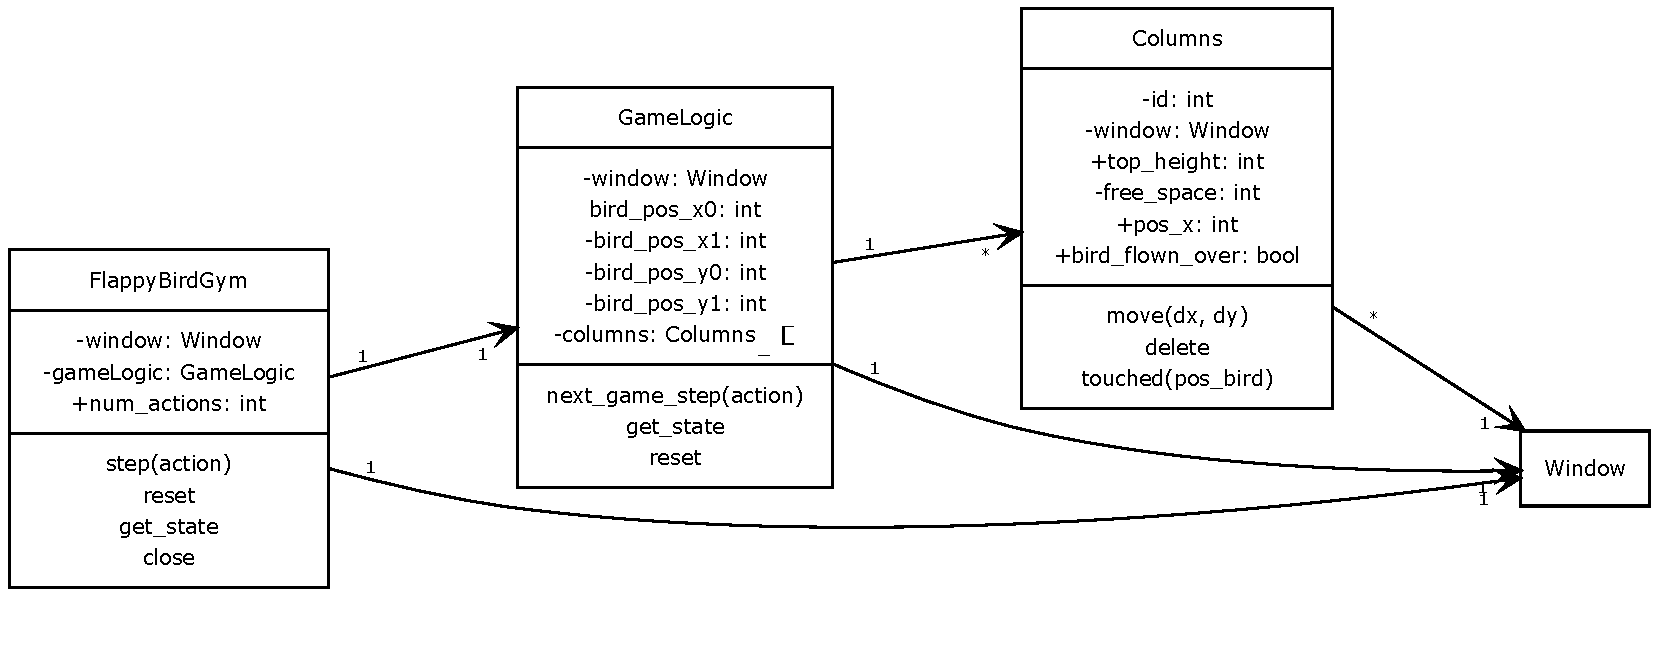
\includegraphics[width=\textwidth]{media/gym.pdf}
    \caption{Environment}
    \label{fig:uml-gym}
\end{figure}

A reference to the window object is passed to each of the mentioned classes. The \mintinline{python}{Window} class implements the graphical representation, which will be explained in further detail in section \ref{sec:ui}.

\subsubsection{Neural Network view}

Given this implementation of the game, what exactly does the state contain that is passed to the neural network? As it can be seen in 
listing \ref{listing:get-state}, for each state 12 parameters are passed to the ANN, which makes 24 in total, since we pass the current and the previous state. These describe the positions of the bird and the two columns which the bird has to pass next. For each of these elements, we pass four parameters, since they have the form of rectangles.
\begin{listing}[!ht]
\begin{minted}{python}
def get_state(self):
    return np.array([
        self.bird_pos_x0, self.bird_pos_y0,
        self.bird_pos_x1, self.bird_pos_y1,
        self.first_column.top_pos_x0, self.first_column.top_pos_y0,
        self.first_column.top_pos_x1, self.first_column.top_pos_y1,
        self.first_column.down_pos_x0, self.first_column.down_pos_y0,
        self.first_column.down_pos_x1, self.first_column.down_pos_y1
    ])
\end{minted}
\caption{get\_state}
\label{listing:get-state}
\end{listing}
The neural networks output is binary, either "flap" or "no flap". It is passed to the environment on each step.
% Network behaviour on a single frame
\subsubsection{Reward function}
In RL it is straightforward to define the outcomes but it is more difficult to define the way to get there.
For instance, in Flappy Bird it is uncomplicated to define how to win the game but it is more complicated to determine how the bird will fly to survive. The bird will simply fly as it rewarded for.
\par
In our reward function, we decided to give the neural network a bit more information than just the game score. In order to pass a gap between two pipes, the bird's vertical position must be between the lowest point of the upper pipe and the highest point of the lower pipe. We wanted to reward our network when this is the case and we did so in the form of a Gaussian reward function which is at it's maximum when the bird is right in the center of the gap.
\par


$reward(x)  
= \frac{\mathcal{N}(x|\mu, \sigma)}{\mathcal{N}(\mu|\mu, \sigma)}  
= \frac{\mathrm{}\frac{1}{\sigma\sqrt{2\pi}} \exp{\biggl(-\frac{(x - \mu)^{2}}{2\sigma^{2}} \biggr)}} 
{\mathrm{}\frac{1}{\sigma\sqrt{2\pi}} \exp{\biggl(-\frac{(\mu - \mu)^{2}}{2\sigma^{2}} \biggr)}}  
= \exp{\biggl(-\frac{(x - \mu)^{2}}{2\sigma^{2}} \biggr)}$

with 

$\mathcal{N}(x|\mu, \sigma) = \mathrm{}\frac{1}{\sigma\sqrt{2\pi}} \exp{\biggl(-\frac{(x - \mu)^{2}}{2\sigma^{2}} \biggr)} $
where  x is $bird\_posY0$; 
\par
Furthermore the reward function is normalized to be between 0 and 1 in order to prevent tiny q values. This is visualized in figure \ref{fig:Rewardsystem}.
\par
The two vertical ordered columns which are the nearest to the bird are considered for the reward calculation. µ denotes the y coordinate of the center of the space between these two columns. 
$\sigma$ denotes the scaled length in y direction of this space. In order to force the model to control the bird more towards the middle the length of the space is scaled by a factor of 0.125.
\begin{figure}
    \centering
    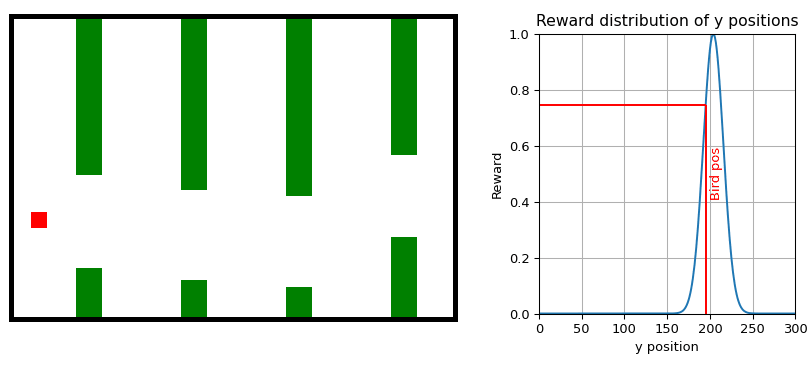
\includegraphics[width=\textwidth]{media/rewardSystem.png}
    \caption{Reward system}
    \label{fig:Rewardsystem}
\end{figure}


%!!Tim fragen wegen Grafik!!


\subsection{Neural Network}

When creating our neural network, we followed the structure we learned during the course. We created a subclass of \mintinline{python}{tf.keras.Model} and implemented the relevant methods \mintinline{python}{__init__}, \mintinline{python}{call} and \mintinline{python}{train_step}. 
% Network overview
\begin{listing}[!ht]
\begin{minted}{shell}
Layer (type)                 Output Shape              Param #   
=================================================================
dense (Dense)                multiple                  1600      
_________________________________________________________________
dense_1 (Dense)              multiple                  8320      
_________________________________________________________________
dense_2 (Dense)              multiple                  129       
_________________________________________________________________
dense_3 (Dense)              multiple                  258       
=================================================================
Total params: 10,307
\end{minted}
\caption{Network summary}
\label{listing:network-summary}
\end{listing}

Since our input data is a small array of numbers (and not the full graphical representation of the game), dense layers suffice to solve the given task (and we do not need any convolutional layers). Listing \ref{listing:network-summary} shows in detail which layers we used. Figure \ref{fig:model-plot} shows the complete network structure, including activation functions.

\begin{figure}
    \centering
    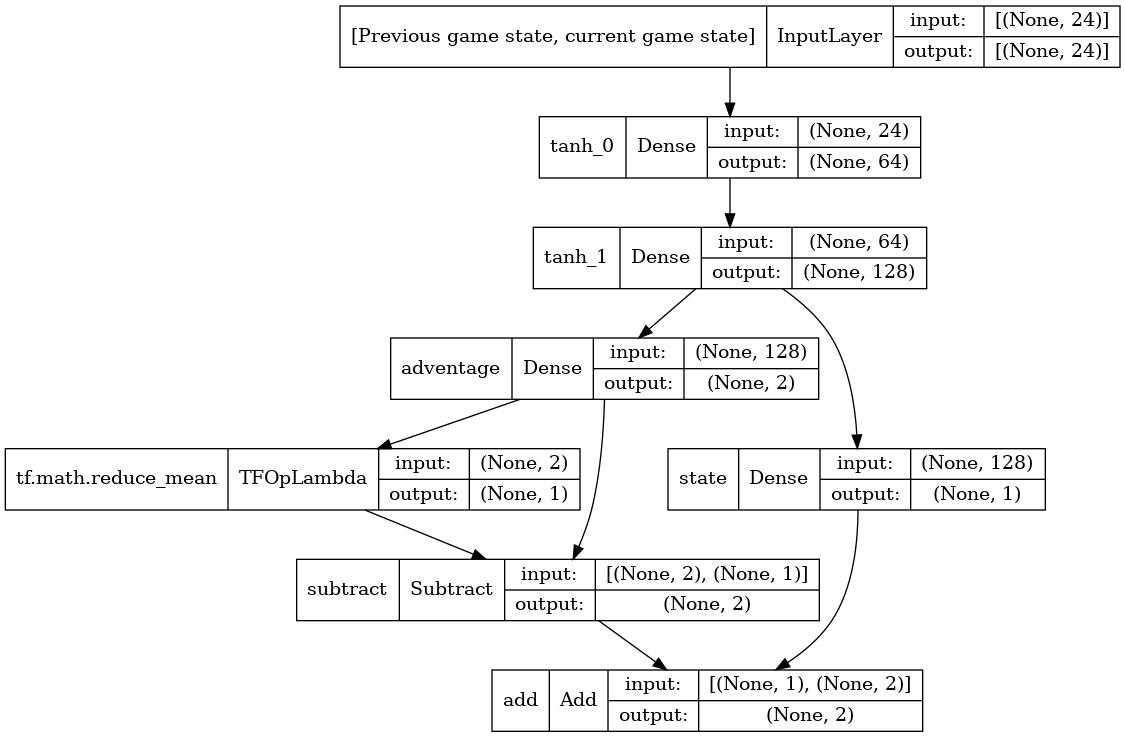
\includegraphics[width=\textwidth]{media/modelPlot.png}
    \caption{Model Plot}
    \label{fig:model-plot}
\end{figure}
\subsection{Hyperparameters}
An important task was to adjust the hyperparameters to obtain the best performance. The choices were not always trivial and we tried several approaches. 
By following the structures we learned in the course but also experimenting with different parameters, in the end we obtained the best performance using the hyperparameters presented in Listing \ref{listing:hyperparams}.


\begin{listing}[!ht]
\begin{minted}{python}

General:
    learning rate = 0.001
    optimizer = Adam
    loss function = mean squared error
    batch size = 32
EpsilonGreedyStrategy:
    start = 1.0 
    end = 0.05
    decay = 0.99 (multiplicative decay after each episode until end is reached)
ReplayMemory:
    capacity = 500.000
    num_samples = 250.000 # number until training the network starts
    sampling process: samples with higher reward preferred
Deep Q Learning:
    gamma = 0.99
    update = 100 # number of episodes when weights of qnet = weights of target net

\end{minted}
\caption{Hyperparameters}
\label{listing:hyperparams}
\end{listing}



\subsection{Double Deep Q-Learning}\label{sec:ddql}

Figure \ref{fig:uml-q-learning} shows how we implemented the Double Deep Q-Learning architecture to let our network learn Flappy Bird. The most superordinate class instance is \mintinline{python}{Training}. It runs the training loop and uses the wrapper classes \mintinline{python}{Agent} and \mintinline{python}{EnvManager} to access the network and the environment. The "Double" of Double Deep Q-Learning is realized by having two neural networks, \mintinline{python}{q_net} and \mintinline{python}{target_net}. In the following, we will describe how these two networks behave during the training loop in detail:
\begin{enumerate}
    \item Filling the replay memory. The untrained network plays the game until the replay memory is filled. When we trained the network, we set the size of the replay memory to 250000.
    \item For each episode:
    \begin{enumerate}
        \item Based on the current exploration rate (which decays over time) and a random value, chose whether the next step will explore or exploit.
        \item Perform a step based on the networks current parameters; if we are exploiting, chose the best option, if we are exploring, chose a random option.
        \item Store the whole step (state before action, action, state after action and reward) in the replay memory.
        \item Perform a training step: Select a sample from the replay memory. Predict the Q-values by both \mintinline{python}{q_net} and \mintinline{python}{target_net}. Compute the maximum Q-value of the next state using the \mintinline{python}{q_net}. The update operation differs a  bit from what we learned during the seminar: We take the action chosen by the \mintinline{python}{q_net} (the action that has the maximum Q-value) and add the expected reward predicted by the \mintinline{python}{target_net} for that exact action to the reward.
        \item Using the state and the computed Q-target (sum of rewards so far and the expected reward described in the previous point multiplied by the discount factor $\gamma$), we can perform a train step on the \mintinline{python}{q_net}.
        \item Repeat these steps for each episode 500 times. After this amount of steps, reduce the exploration rate.
    \end{enumerate}
    \item After 100 episodes, copy the current \mintinline{python}{q_net} to be the new \mintinline{python}{target_net}. In total, we run 5000 episodes.

\end{enumerate}
\par
\begin{figure}
    \centering
    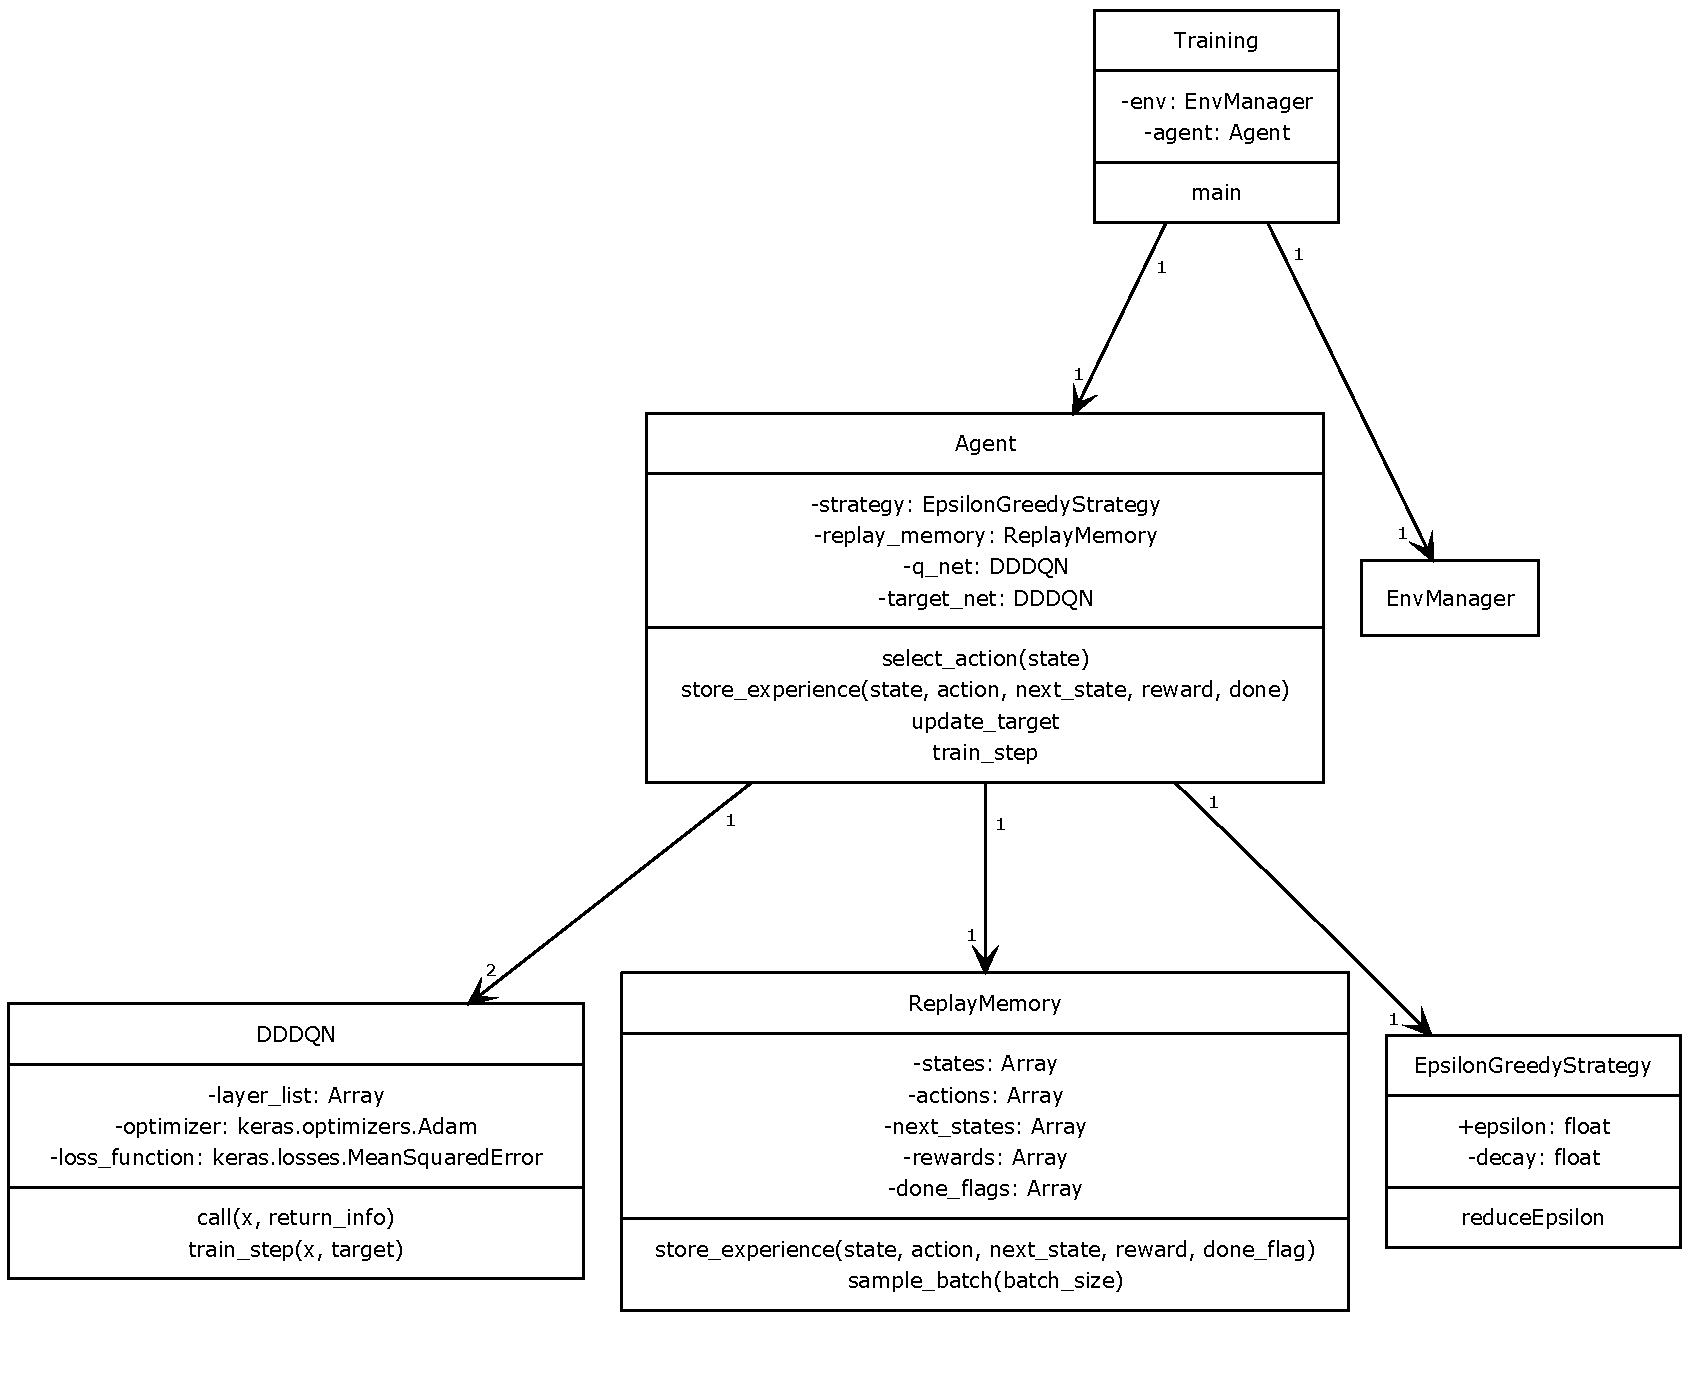
\includegraphics[width=\textwidth]{media/network.pdf}
    \caption{Double Deep Q-Learning}
    \label{fig:uml-q-learning}
\end{figure}


\subsection{User Interface}\label{sec:ui}

We developed three different modes of running our network:
\begin{enumerate}
    \item No window
    \item Game window
    \item Game + Stats window
\end{enumerate}
The no window-mode runs without GUI, although some information are passed to the user via command line. We used that mode for training, since it runs the fastest.
\par
The game window mode shows the actual game of Flappy Bird with the network-controlled bird. Compared to the no-window mode, the user can see how the bird is behaving, which can be used to troubleshoot problems if the network is not learning.
\par
Even more information are contained in the game + stats window mode (see figure \ref{fig:stats-window}), where in addition to the game itself also the internal game state and network behaviour is displayed. The top three plots show which action is currently seen as the best by the network, the current reward distribution in relation to the bird's height and the so far obtained rewards. In the bottom row, the UI shows the 12 inputs of the current state and the activations of the layers 1 and 2. On the left, we can see our graphical representation of the game itself which also looks the same in the game window mode.

\begin{figure}
    \centering
    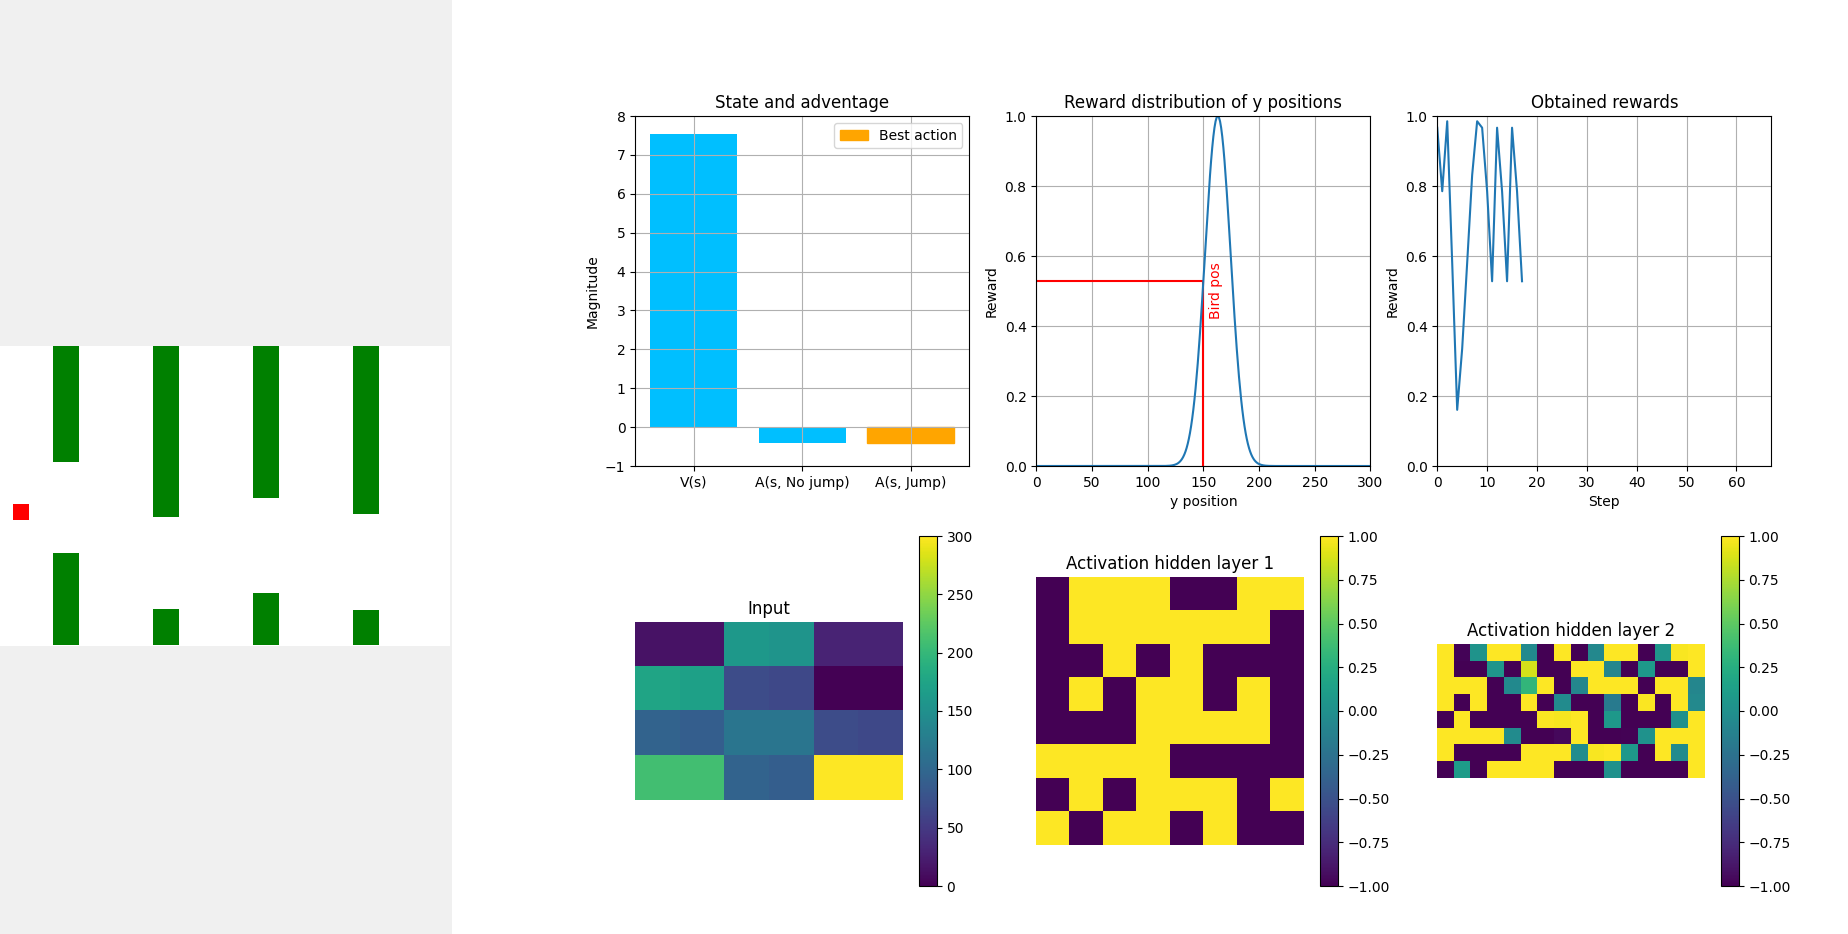
\includegraphics[width=\textwidth]{media/Screenshot-stats-window.png}
    \caption{Game + Stats Window Mode}
    \label{fig:stats-window}
\end{figure}

\section{Evaluation}\label{sec:eval}

\subsection{Analysis of results}

As a result of our project, we managed to implement an ANN that uses deep reinforcement learning to learn playing the game Flappy Bird. We used a technique called "Double Deep Q Learning" to go beyond what we learned during the course. Apart form the mere fact that the network learned to play the game, we also gained some insights which we regard as the true learning success of this paper and we will present in the following.
\par
First, by building the environment ourselves, we learned how big of a role the environment and by that the possible inputs into a network play. At the beginning, we naively created our environment and thought that from that moment on, the task would only lie in finding the neural network architecture to work. But during the course of the project, we realized that tweaks to the environment can have a far greater influence on the networks learning behaviour. A prime example is how we implemented the reward: Our first version of the program gave the reward 1 if the bird passed a pipe, -1 if it hit a pipe or left the playing field and 0 for every other state. That led to a situation where the for almost all states, no reward could be gained. No matter how we tweaked our network, it did not learn. Only by changing the reward function into its current state, that the ANN receives positive reward if it is on the same height as the gap between the pipes, we could solve the issue of not learning. Giving the reward a Gaussian shape with the maximum at the center of the gap further increased the learning ability of the network.
\par
We also learned a lot by using a more sophisticated learning algorithm in the form of our Double Deep Q-Learning algorithm. We already learned architectures that use multiple ANNs during our course (for instance using an encoder and decoder to generate images), but still it was an interesting learning how a combination of multiple ANNs can improve the overall learning performance.
\par
Both these insights led to the more general insight: The singular network itself is not as important in deep learning as we thought it to be. The number and size of layers influences learning, but a changing what surrounds the network can also have a very significant influence. 
\par
In the following, we will evaluate the network in greater (technical) detail.

\subsection{Training}

As shown in Figure~\ref{fig:training-plot}, during training the average reward, epsilon magnitude, score and steps per episode were monitored.  
Score denotes the sum of all obtained rewards within a episode.
Note that the number of episode does not include the necessary episodes to fill the replay memory.
Before the actual training (changing network weights) begins, 250000 training samples (also called experiences) must be stored in the replay memory.
After about 400 episodes, the average reward decreases. 
However, at 600 episodes the average reward increases again.
Score and steps per episode increases over the entire training episodes.
Overall, the decrease of the average reward is irrelevant due to the actual goal: The model shall live (no collision with a column) as long as possible.
In other words, the goal was to increase the steps per episode.

\begin{figure}[h]
    \centering
    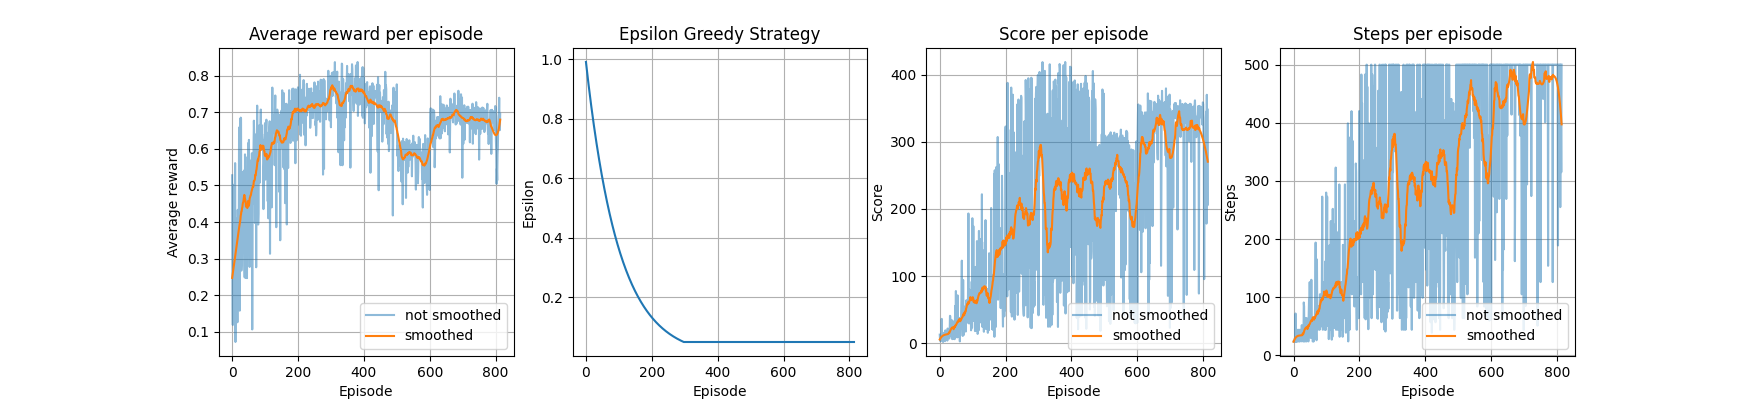
\includegraphics[width=\textwidth]{media/trainingPlot.png}
    \caption{Average reward, epsilon magnitude, score and steps per episode monitored during training.}
    \label{fig:training-plot}
\end{figure}

\subsection{Model Performance}

Figure~\ref{fig:performance-plot} presents the obtained rewards for 250 steps of the previously described model after tranining has finished. 
In average the model receives a reward of 0.8, which is rather high.
A collision with a column never occurred.
The downwards spikes of rewards followed with an immediate increase is caused by our reward calculation: Whenever the bird passes a column gap, the reward immediately is calculated for the next obstacle, which has a different height.
Since the model tries to maximize its reward by controlling the bird to be on the same height as the gap between the upcoming pipes, it vertically moves the bird towards the optimal position. 
As a consequence, the reward increases again.
\par
The small oscillations in reward are explained by the physical behaviour of the bird: It is always in the state of falling, and when the agent "flaps", it leaps upwards a certain height. 

\begin{figure}[h]
    \centering
    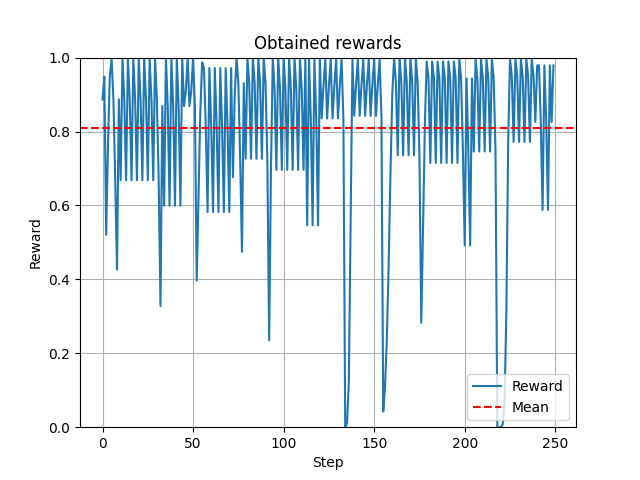
\includegraphics[width=\textwidth]{media/performancePlot.png}
    \caption{Running the model for 250 episodes.}
    \label{fig:performance-plot}
\end{figure}

\subsection{Comparison to related approaches}
As described in section \ref{sec:related}, there have been several related approaches, but only the one by Chen (\cite{chendeep}) has a similar focus as our project, as the others either use very different architectures (genetic algorithm) or have a different focus (as in \cite{performanceFB}. Hence, we will compare our project only to the former approach.
\par
One big difference between our approach and the one by Chen is the state. Chen passes the current frame, the current point in time and a parameter that dictates how many past frames have to be considered, while we only pass two times (current and past state) the 12 parameters as shown in listing \ref{listing:get-state}. Because of that, the network structure also differs: In order to process pixel-wise information, Chen uses convolutional layers which we do not need.
\par
Apart from these differences, the learning itself is rather similar. Chen does use not use the exact same Double Deep Q-Learning algorithm we use, although as described in section "Stability" \cite[p. 3]{chendeep}, he also uses an additional target network. The result is the same as ours, namely that the network learns to play the game.
\section{Conclusion}

The goal of our project was the application of our acquired skills to a new problem, for which we chose the game "Flappy Bird". We decided to use deep reinforcement learning, more specifically Double Deep Q-Learning as an architecture to solve the problem. We created a working environment and an agent which used that environment to learn the game. In this task, we were successful. We also put our work into the greater context of scientific background knowledge, related work and evaluated it.  

\par
Beyond this general conclusion, we would also like to draw a more personal one: During the project, we experienced our first complete deep learning project, encountered many new things, overcame difficulties and had a great learning success. Insofar, the project was a nice ending of the IANNwTF course. 


\newpage
\printbibliography

\end{document}

